\documentclass{article}


\usepackage{times}
\usepackage{url}
\usepackage{amsfonts,amssymb}
\usepackage{color}

\usepackage{amsmath}
\usepackage{acronym}
\usepackage{xspace} % mellemrum efter forkortelser fra acronym package.
\usepackage{graphicx,graphics,colortbl}

\definecolor{gray1}{rgb}{0.9,0.9,0.9}
\definecolor{gray2}{rgb}{0.75,0.75,0.75}
\definecolor{gray3}{rgb}{0.6,0.6,0.6}

\newcommand{\xcell}[2]{{\cellcolor{#1}#2}}
\newcommand{\ffh}[1]{{\color{red} #1}}

\usepackage{algorithmicx}
\usepackage[noend]{algpseudocode}
\usepackage{algorithm}

\usepackage{cite}

\sloppy
% correct bad hyphenation here


\newtheorem{definition}{Definition}
\newtheorem{problem}{Problem}
\newtheorem{lemma}{Lemma}

\newcommand{\todo}[1]{\textbf{TODO: \color{red}{#1}}}

\begin{document}

\pagestyle{plain}
 \title{Simpler directions via Shortcuts}

\maketitle

\begin{abstract}
abstract
\end{abstract}


\acrodef{SP} {Shortest Path}


\section{Problem}

We first provide definitions and define concepts.% Then we define our optimization problem.

\begin{definition}[Graph] \label{def:graph}
Let $G(V, E, W)$ be a directed spatial graph with a set $V$ of nodes and a
set $E \subseteq V \times V$ of edges.
Each node $v_i \in V$ models a road junction and has lat-long coordinates.
Each edge $(v_i, v_j) \in E$ models a road segment, and $W$:$E \rightarrow R$
assigns a positive weight to each edge.
\end{definition}
%For simplicity, we consider $G$ to be an undirected graph.
%Our proposed methods can be easily adapted for directed graphs.


\begin{definition}[Familiar Road] \label{def:froad}
A familiar road $F_{s,t}$ is a set of connected edges from s to t
which a user has traversed in the past.
\end{definition}


\begin{definition}[Shortcut] \label{def:shortcut}
%
A shortcut $S_{s,t}$ is a path $P_{s,t}$ from s to t which includes
at least one familiar road $F_{a,b}$, where a and b are vertices on
the path $P_{s,t}$ and $dist(S_{s,t}) \leq SP_{s,t} \ast (1+\epsilon)$.
$dist(S_{s,t})$ is the sum of the edge weights from s to t.

Each $F_{a,b}$ is connected to $P_{s,t}$ via a pair of connecting paths $c_{a1,a2}, c_{b1,b2}$.
The part of $P_{a,b}$, covered by $F_{a,b}$, is not used
\end{definition}

\begin{problem}[Ideal Shortcut] \label{def:idealshortcut}
We want to find an \textit{Ideal Shortcut} $IS_{s,t}$. 
$IS_{s,t}$ is $min(|S_{s,t}|) || S_{s,t} \in \mathcal{S}$, where $\mathcal{S}$ 
is the set of all $S_{s,t}$. $min(|S_{s,t}|)$ denote the path with the fewest 
vertices.
\end{problem}


As an example see figure \ref{fig:shortcutex}. Conceptually the idea is to 
replace part of a shortest path with a path that is familiar to the user. This 
is illustrated in the top part of figure \ref{fig:shortcutex}. 
What we then do is identify a useful subpath of a, previously traversed, familiar 
path and add a shortest path from the original start and end points (s,t), to the 
start and end points (a,b) of the familiar path, as seen in the lower part of figure
\ref{fig:shortcutex}.

\begin{figure}[Bht]\label{fig:shortcutex}
\center
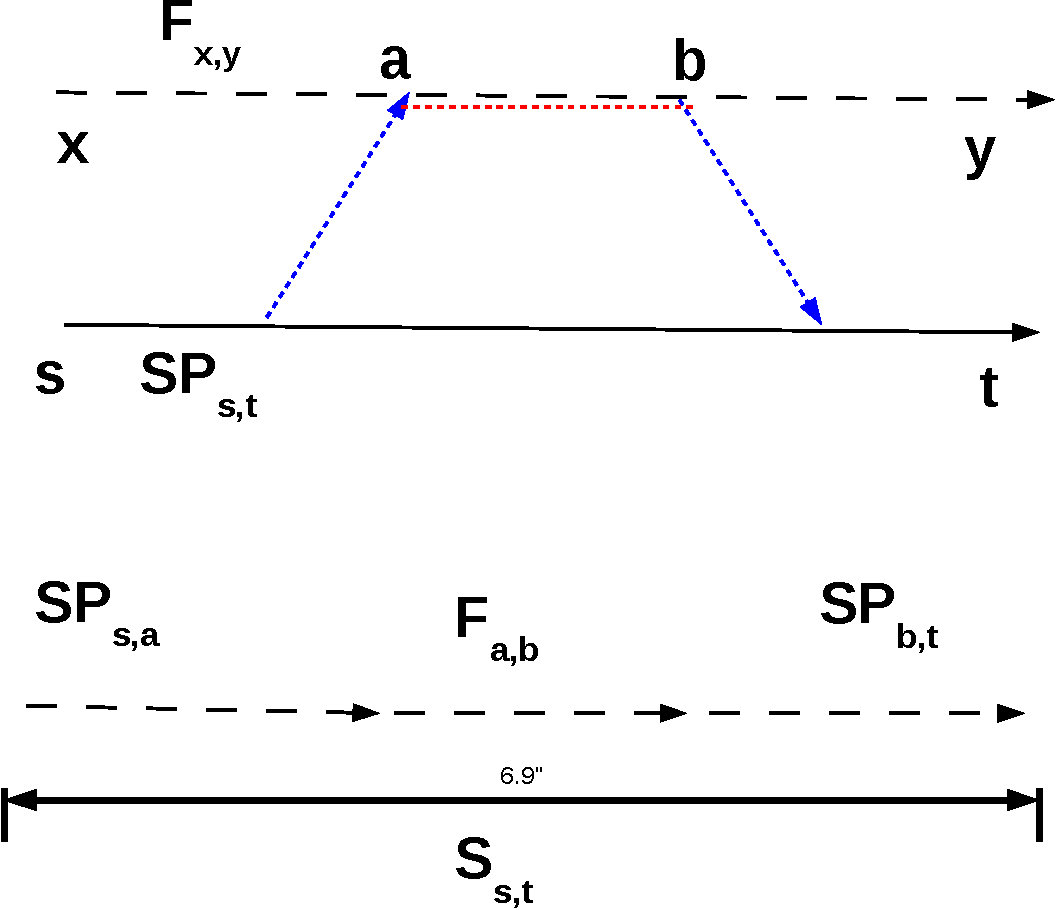
\includegraphics[width=0.78\columnwidth]{figures/shortcut} 
\caption{shortcut example}
\end{figure}


A naive solution to finding an Ideal Shortcut $IS_{s,t}$ is to first run dijkstra 
on a graph from both $s$ and $t$, to get two shortest path trees $T_s$ and $T_t$. 
Then, try to find any familiar paths $F_{a,b}$ with $a$ intersecting in $T_s$ 
and $t$ intersecting in $T_t$. A familiar path may intersect multiple times with 
both $T_s$ and $T_t$.

After all possible combinations are found the Ideal Shortcut can easily be identified
by picking the shortest path among all the combinations.

The algorithm for the naive solution is outlined in algorithm \ref{alg:naiveshortcut}.
Line 5 and 6 prune the number of possible $F_{a,b}$ to be examined by implementing 
the observation from lemma \ref{lem:sacondition}.

\begin{lemma}\label{lem:sacondition}
If $dist(SP_{s,a})$ is greater than $dist(SP_{s,t})$ no $dist(F_{a,b})$ exist
which satisfies $dist(SP_{s,a}) + dist(F_{a,b}) + dist(SP_{b,t}) \leq dist(SP_{s,t}) \ast (1+\epsilon)$
\end{lemma}

\begin{algorithm}[hbt]
\small
\caption{\label{alg:naiveshortcut} {\bf Naive Shortcut}(Query $Q_{s,t}$, Graph $G(V,E)$, tuning parameter $\epsilon$, Familiar roads $\mathcal{F}$)}
\begin{algorithmic}[1]
  \State run Dijkstra on G from both s and t; \Comment{Get all $dist(s,v)$ and $dist(v,t)$ for all vertex $v$}
  \State $\mathcal{SC}_{s,t} \leftarrow SP_{s,t}$ \Comment{Ideal Shortcut candidate with fewest vertices}
  \For{{\bf each} $F_{x,y} \in \mathcal{F}$}
    \For{{\bf each} $a \in F_{x,y}$}
      \If{$dist(SP_{s,a}) \geq dist(SP_{s,a}) \ast (1+\epsilon)$} 
	\State Skip current iteration  %\Comment{equivalent to "continue"}
      \EndIf
      \For{{\bf each} $b \in F_{x,y} | a < b$}
	\If{$dist(SP_{s,a}) + dist(F_{a,b}) + dist(SP_{b,t}) \leq dist(SP_{s,t}) \ast (1+\epsilon)$}
	  \If{$|SP_{s,a}| + |SP_{b,t}| < |\mathcal{SC}_{s,t}|$}
	    \State $\mathcal{SC}_{s,t} \leftarrow \left(SP_{s,a}, F_{a,b}, SP_{b,t} \right)$
	  \EndIf
	\EndIf
      \EndFor
    \EndFor
  \EndFor
  
  \State {\bf Return} $\mathcal{SC}_{s,t}$;
\end{algorithmic}
\end{algorithm}


\clearpage
\vspace{2em}
good ideas
\begin{itemize}
\item Store intersections with $T_s$ and $T_t$ in maps for efficiency 
\item A familiar path can obviously intersect many times, do not include 
intersections that result in longer paths than have already been found.
\item Do not run full Dijkstra on graph, limit to area between s and t for a 
path $P_{s,t}$. -- Use heuristic, maybe run an A* 
\item using $\epsilon$ it is possible to restrict the search space for possible 
$F_{s,t}$ intersections significantly

\end{itemize}

\todo{what to do with $\#F_{a,b} > 1$?}
\todo{make basic algorithm better than naive}
\todo{make psudo code for algorithm for $\#F_{a,b} > 1$}



% \section{NOTES}
% 
% \begin{enumerate}
%   \item condition: $dist(S_{s,t}) \leq SP_{s,t} \ast 1+\epsilon$
%   \item minimize: $|P_{s,t} |$ -- \# vertices
%   \begin{itemize}
%     \item $ = |P_{s,c1}| + |C1| + |C2| + |P_{c2,t}| = |SP_{s,a}| + |SP_{b,t}| $
%   \end{itemize}
%   \item Algorithm
%   \begin{itemize}
%     \item [1.]
%     \item [2.] extract
%     \item [3.] Prune
%   \end{itemize}
% \end{enumerate}
% 
% write down condition and minimization problem tidily
% 
% write algorithms for naive solution
% 
% maybe - write down some more interesting solution and algorithm/figure for it.

\end{document}




